% Figure from MATH 556 notes, section 20. Compile with the notes preamble.
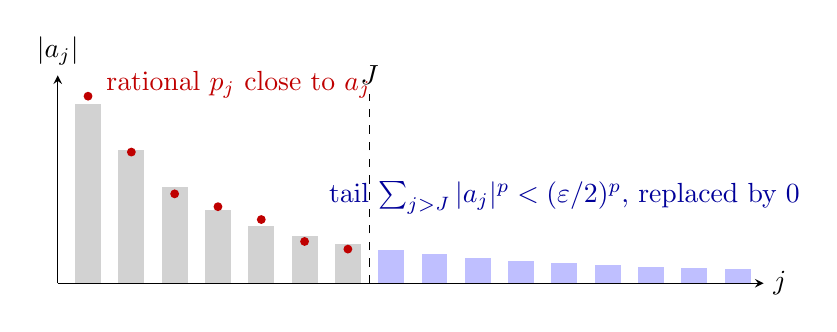
\begin{tikzpicture}[x=0.55cm, y=2.4cm, >=stealth]
    \draw[->] (0.3,0) -- (16.6,0) node[right] {$j$};
    \draw[->] (0.3,0) -- (0.3,1.1) node[above] {$|a_j|$};
    \foreach \j in {1,...,16} {
        \pgfmathsetmacro{\h}{0.95/(1+0.35*(\j-1)^1.3)}
        \ifnum\j<8
            \fill[gray!35] (\j-0.3,0) rectangle (\j+0.3,\h);
            \fill[red!75!black] (\j,{\h+0.04*sin(97*\j)}) circle (1.6pt);
        \else
            \fill[blue!25] (\j-0.3,0) rectangle (\j+0.3,\h);
        \fi
    }
    \draw[dashed] (7.5,0) -- (7.5,1.0) node[above] {$J$};
    \node[red!75!black, anchor=west] at (1.2,1.05) {rational $p_j$ close to $a_j$};
    \node[blue!60!black] at (12,0.45) {tail $\sum_{j > J} |a_j|^p < (\varepsilon/2)^p$, replaced by $0$};
\end{tikzpicture}
